\documentclass{foi}
\usepackage[utf8]{inputenc}
\usepackage{lipsum}

\vrstaRada{\projekt} % \diplomski \projekt \seminar \zavrsni
\title{Aplikacija za vođenje statistike skladišta i planiranje zaliha}

\author{Antonio Grgošević}
\spolStudenta{\musko} % \zensko ili \musko
\mentor{Bogdan Đurić Okreša}
\spolMentora{\musko} % \zensko ili \musko
\godina{2020}
\mjesec{lipanj}
\date{2020}
%\status{redoviti}
\indeks{44264/15–R}
\smjer{Organizacija poslovnih sustava} % (ili Poslovni sustavi, Ekonomika poduzetništva, Primjena informacijske tehnologije u poslovanju, Informacijsko i programsko inženjerstvo, Baze podataka i baze znanja, Organizacija poslovnih sustava, Informatika u obrazovanju)
\titulaProfesora{Dr. sc.}

\sazetak{Izrada aplikacije koja koristi bazu podataka s aktivnim i temporalnim komponentama. Izrađena aplikacija namijenjena je za vođenje statistike skladišta i upravljanje zalihama koje su na skladištu FIFO strategijom.}

\kljucneRijeci{aktivna baza podataka, temporalna baza podataka, skladište, implementacija, FIFO strategija, PostgreSQL}

\begin{document}

\maketitle

\tableofcontents

\pagestyle{plain}
\chapter{Opis aplikacijske domene} % \Opis aplikacijske domene

U ovom poglavlju biti će opisana detaljnije aplikacijska domena sustava.
Izrađena aplikacija je namijenjena za vođenje statistike skladišta i upravljanje zalihama koje su na skladištu. 
Sama struktura aplikacijske domene sastoji se od sljedećih elemenata:
\begin{itemize}
    \item Artikl
    \item Zaposlenik
    \item Kupac
    \item Dobavljač
    \item Narudžba
    \item Radni nalog
    \item Stanje na skladištu
\end{itemize}

Prvenstveno je važno napomenuti da aplikacijom upravlja zaposlenik koji unosi određene artikle koje se može naručiti, a poslije i prodati kupcu. Skladište funkcionira na način da se prvo naruči određena količina artikala koji onda pristižu na skladište. Pri tome se vodi računa o tome koji zaposlenik je izdao određenu narudžbu, od kojeg dobavljača i na koji datum. 

Jedan artikl može biti podijeljen na više paketa, pa se zbog toga artikli naručuju u paketima.
Nakon što određeni artikl pristigne na skladište, a pristigne nakon što je izdana narudžba, na stanju na skladištu mu se povećava trenutna količina. Prethodno opisani način zapravo predstavlja ulazak artikla na skladište. Kako bi određeni artikl bio prodan kupcu, odnosno kako bi izašao sa skladišta, potrebno je da zaposlenik unese radni nalog. Prilikom unosa radnog naloga potrebno je da se odabere zaposlenik, koji izdaje taj radni nalog te kupac kojem se izdaje radni nalog. Osim toga potrebno je da zaposlenik unese količinu koja će biti izdana te da odabere točan datum izdavanja radnog naloga. Nakon što je radni nalog izdan, stanje na skladištu mu se smanjuje za izdanu količinu.

\chapter{Teorijski uvod} % \Teorijski uvod

Izrađena aplikacija koristi aktivnu i temporalnu bazu podataka. U sljedeća dva potpoglavlja će iste biti opisane.
\section{Aktivna baza podataka}
Aktivne baze podataka ne samo da pohranjuju podatke i informacije, već reagiraju na događaje i provode akcije prema tim događajima, npr. umetanje podataka, brisanje podataka, ažuriranje podataka i slično. Aktivno ponašanje u bazi podataka se postiže definiranjem pravila „Događaj-Uvjet-Akcija“. Pojava događaja pokreće procjenu uvjeta te ako se uvjet procjeni istinitim, tada se radnja izvršava. Možemo reći da pravovremeno reagiraju na novonastale situacije [1].

\section{Temporalna baza podataka}
Temporalna baza podataka pohranjuje podatke koji se odnose na vremenske instance.  Nudi vremenske tipove podataka i pohranjuje podatke koji se odnose na prošlo, sadašnje ili buduće vrijeme. Temporalna baza podataka pohranjuje zbirku vremenski povezanih podataka. Povezivanjem vremena s podacima, moguće je pohraniti različita stanja baze podataka [2].

\chapter{Model baze podataka} % \Model baza podataka

Model baze podataka prikazan je preko ERA modela u kojem se nalaze sve potrebne tablice i veze između njih. ERA model izrađen je u MySQL Workbench aplikaciji jer je vrlo jednostavna za korištenje i kreiranje tablica. Osim toga nudi automatsko kreiranje slabih entiteta koji su prijeko potrebni u ovom projektu. Na slici 1. prikazan je izrađeni ERA model. \begin{figure}[h]
    \centering 
    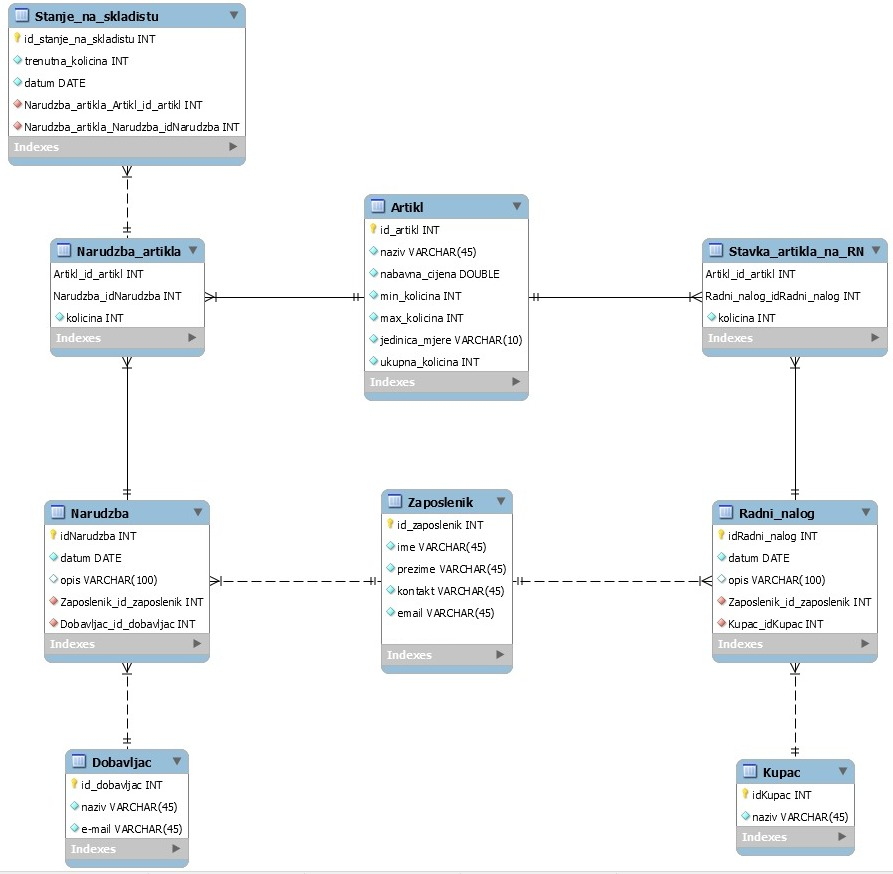
\includegraphics[width=1.0\textwidth]{slike/ERA.jpeg}
    \caption{Prikaz ERA modela baze podataka}
    \label{slika-1}
\end{figure}

Na slici 1. vidljivo je kako se baza podataka sastoji od 7 tablica i 2 slaba entiteta. Slabe entitete predstavljaju    \emph{Narudzba artikla} i \emph{Stavka artikla na RN}, odnosno to su tablice koje se kreiraju na vezama više na više.
\newpage
\section{Zaposlenik}
U tablici Zaposlenik nalaze se podaci o svim zaposlenicima koji mogu upravljati skladištem, a samim time i aplikacijom. Svaki zaposlenik ima svoje ime i prezime, kontakt broj i email. Glavna svrha zaposlenika je unos svih narudžbi i radnih naloga. Na taj način se uvijek zna koji zaposlenik je unio određenu narudžbu ili radni nalog.

\section{Dobavljač}
U tablici Dobavljač nalaze se svi podaci o dobavljačima od kojih se naručuju artikli. Dobavljač ima svoj naziv te email ukoliko ga je potrebno kontaktirati.

\section{Kupac}
Tablica Kupac sadrži osnovne podatke o svim mogućim kupcima, odnosno sadrži njihov naziv. Nakon što se određeni artikl naruči od dobavljača, on pristiže na skladište te se potom prodaje kupcima. 

\section{Artikl}
Tablica Artikl sadrži sve podatke o artiklima na skladištu. Svaki artikl ima svoj naziv, cijenu po kojoj se on nabavlja i jedinicu mjere. Također sadrži još i informacije koliko minimalno i maksimalno može biti određenog artikla na skladištu te kolika je ukupna količina svih paketa određenog artikla. Kod unosa artikla, ukupna količina je uvijek 0 te se ista mijenja prilikom izdavanje narudžbe ili radnog naloga.

\section{Narudžba}
Tablica Narudžba sadrži sve potrebne informacije o pojedinim narudžbama. Najvažniji podatak kod narudžbe je datum, koji predstavlja datum kada je određena narudžba izdana. Također sadrži i opis narudžbe ukoliko je potrebno nešto posebno napomenuti. Na nju se povezane tablica Zaposlenik i Dobavljač kako bi se znalo koji je zaposlenik izdao narudžbu i od kojeg dobavljača.

\section{Narudžba artikla}
Ova tablica predstavlja slabi entitet koji služi za dodavanje artikala na narudžbu. Tu se zapisuje količina koja se naručuje za svaki artikl te se za tu količinu povećava trenutna količina artikl na stanju na skladištu. Samim time ova tablica je povezana s tablicom Stanje na skladištu i Artikl.

\section{Radni nalog}
Tablica Radni nalog sadrži sve informacije o pojedinim radnim nalozima te se koristi kao izlazak artikla sa skladišta, odnosno za smanjivanje količine pojedinog artikla. Sadrži podatke o opisu i datumu izdanog radnog naloga. Povezana je s tablicom Zaposlenik i Kupac kako bi se znalo koji zaposlenik je izdao radni nalog i kojem kupcu. Osim toga povezana je i s tablicom Stavka artikla na radni nalog koja će biti detaljnije opisana u idućem potpoglavlju. 

\section{Stavka artikla na Radni nalog}
Ova tablica predstavlja slabi entitet koji se koristi kako bi pojedini artikl mogao izaći sa skladišta, odnosno kako bi se prodao određenom kupcu. Sukladno tome, povezana je s tablicom Artikl i Radni nalog preko vanjskih ključeva te u sebi sadrži količinu za koju se pojedini artikl smanjuje sa skladišta. 

\section{Stanje na skladištu}
Ova tablica služi za evidenciju trenutnih količina svakog dostupnog artikla. Trenutna količina se povećava ili smanjuje, ovisno o tome je li izdana narudžba ili radni nalog. Osim toga sadrži i datum koji predstavlja točan datum kada je pojedini artikl dospio na skladište, odnosno kada je naručen.

\chapter{Implementacija}

Baza podataka izrađena je u PostgreSQL-u i za to je korišten alat pgAdmin 4. Sve tablice i veze među njima se kreiraju preko grafičkog sučelja odabirom opcija. Iz tog razloga nije bilo potrebno ručno pisati SQL kod za isto.

\section{Korištenje aplikacije}

Kako bi se aplikacija i baza podataka instalirale potrebno je napraviti sljedeće:
\begin{itemize}
    \item Preko setup datoteke instalirati aplikaciju na željeno mjesto
    \item Na lokalno serveru od izabrane postgres baze podataka kreirati korisnika \emph{admin}  s lozinkom \emph{admin} i postaviti ga na superuser, odnosno dati mu sva dopuštenja
    \item U nekoj od postgres baza podataka kreirati bazu podataka s imenom \emph{TBP Baza} (preporučeno je koristiti pgAdmin 4)
    \item Otvoriti datoteku SkladisteBackUp.sql te kopirati njezin sadržaj u prozoru za izvršavanje SQL upita
\end{itemize}

U  nastavku ovog poglavlja bit će prikazane slike kreiranja prethodno navedenih koraka u alatu pgAdmin 4.
\newline
\begin{figure}[h]
    \centering 
    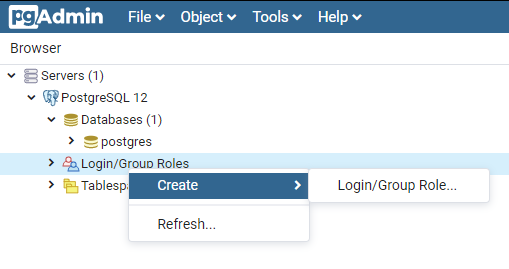
\includegraphics[width=0.7\textwidth]{slike/kreiranje novog korisnika.PNG}
    \caption{Prikaz opcije za kreiranje novog korisnika}
    \label{slika-2}
\end{figure}

\newpage
Na slici 3. vidljiv je prikaz prozora za kreiranje novog korisnika pod nazivom \emph{admin}. U kartici privilegije dane su mu sve privilegije čime je zapravo postao superuser.

\begin{figure}[h]
    \centering 
    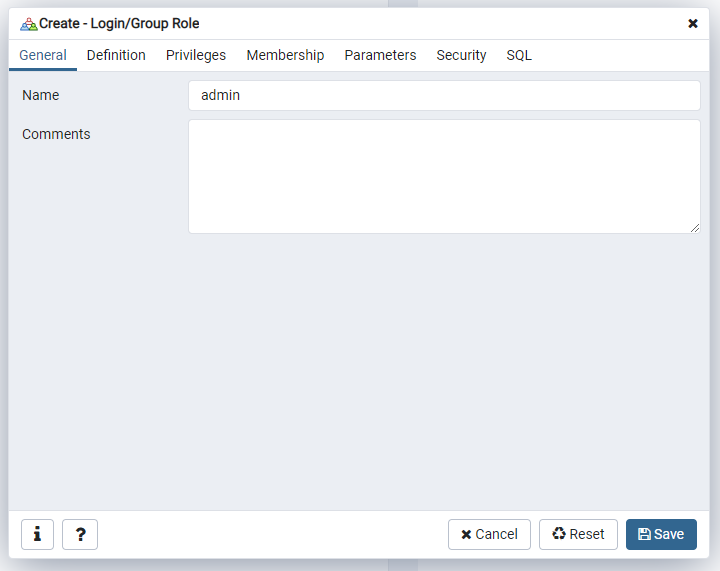
\includegraphics[width=0.65\textwidth]{slike/Ime korisnika - admin.PNG}
    \caption{Ime korisnika - admin}
    \label{slika-3}
\end{figure}
Na slici 4. vidljiv je prikaz dijela kod definiranja lozinke. Korisniku \emph{admin} zbog jednostavnosti je dana identična lozinka imenu korisnika, odnosno lozinka je \emph{admin}.
\begin{figure}[h]
    \centering 
    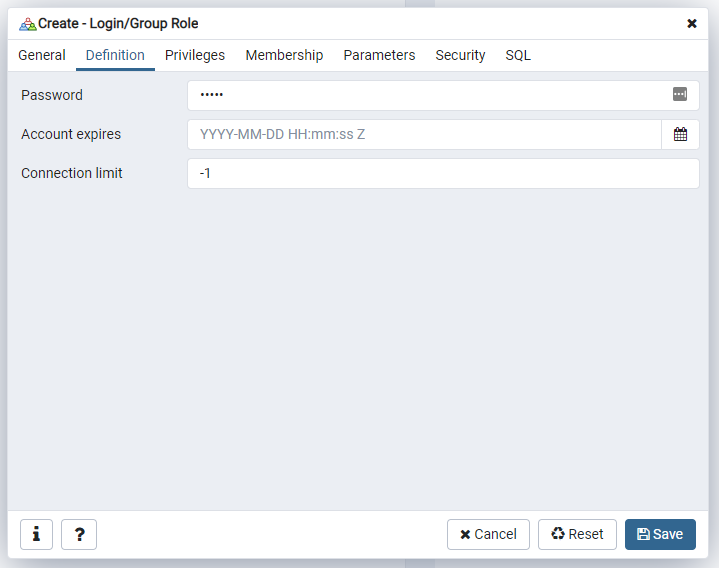
\includegraphics[width=0.65\textwidth]{slike/lozinka za admina(admin).PNG}
    \caption{Lozinka korisnika - admin}
    \label{slika-4}
\end{figure}

\newpage
Na slici 5. vidljiv je prikaz izbornika u kojem desnim klikom na Databases je moguće kreirati novu bazu.
\begin{figure}[h]
    \centering 
    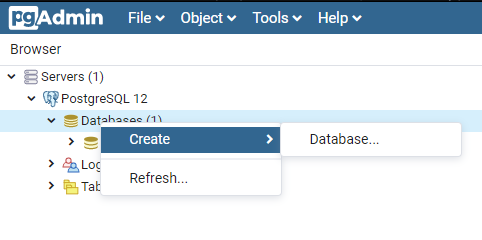
\includegraphics[width=0.7\textwidth]{slike/kreiranje baze.PNG}
    \caption{Kreiranje baze podataka}
    \label{slika-5}
\end{figure}

Na slici 6. vidljiv je prikaz danog imena baze podataka za ovaj projekt pod nazivom \emph{TBP Baza}

\begin{figure}[h]
    \centering 
    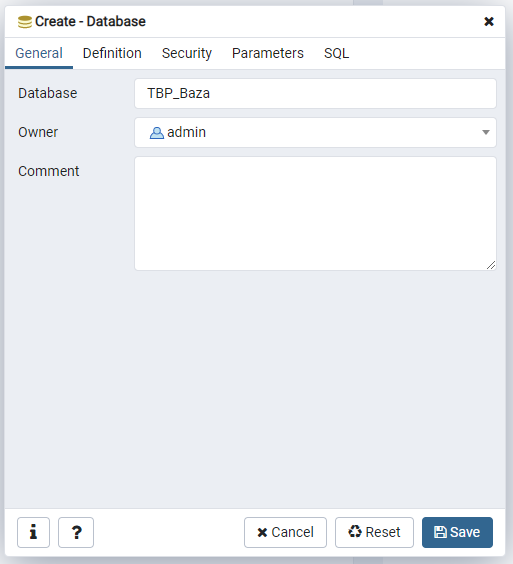
\includegraphics[width=0.5\textwidth]{slike/ime baze.PNG}
    \caption{Ime baze podataka - TBP Baza}
    \label{slika-6}
\end{figure}

\newpage
Na slici 7. prikaz je prozor za backup kreirane baze podataka. Potrebno je odabrati datoteku, pod nazivom \emph{SkladisteBackUp}, u kojoj će biti pohranjene sve kreirane tablice, okidači i funkcije. 
\begin{figure}[h]
    \centering 
    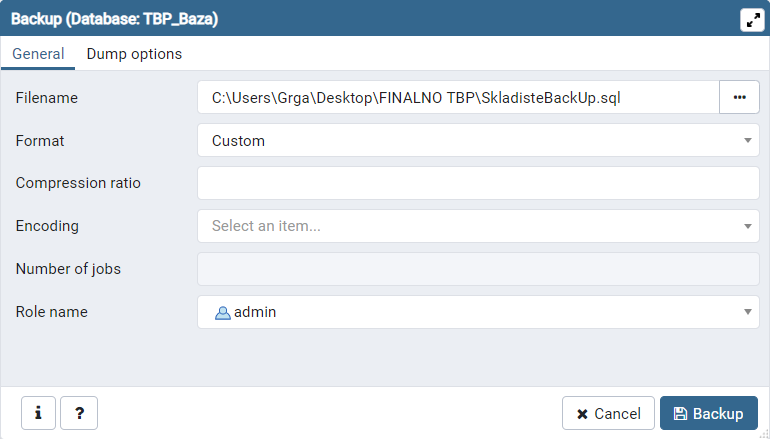
\includegraphics[width=0.9\textwidth]{slike/Back up baze podataka.PNG}
    \caption{Backup baza podataka}
    \label{slika-7}
\end{figure}

Na slici 8. vidljiv je prozor za restore baze podatka. Tu je također potrebno odabrati datoteku, pod nazivom \emph{SkladisteBackUp}. Pritiskom na gumb Restore, ubacit će se kreirana baza podataka te sve njezine povezane tablice, okidači i funkcije. 

\begin{figure}[h]
    \centering 
    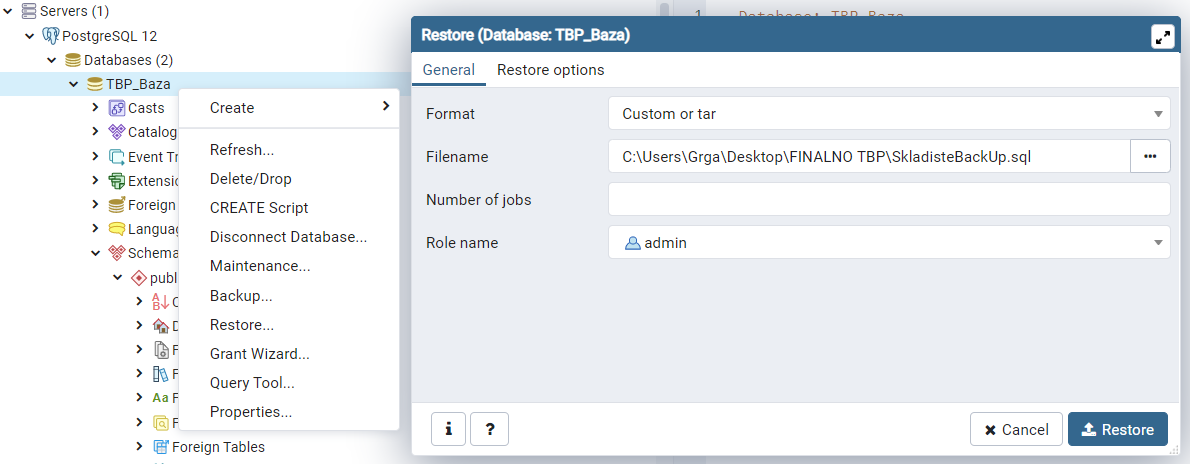
\includegraphics[width=1.1\textwidth]{slike/Restore baze podataka.PNG}
    \caption{Restore baza podataka}
    \label{slika-8}
\end{figure}

\newpage
\section{Implementirane funkcije}
U iduća dva potpoglavlja će biti prikazane dvije izrađene funkcije te će biti objašnjena njihova svrha u aplikaciji.
\subsection{Funkcija za dodavanje nove narudžbe}
Prvenstveno je kreirana funkcija za dodavanje nove narudžbe. Obzirom da je potrebno prvo dodati podatke u tablicu Narudžbu, a tek onda u slabi entitet, odnosno tablicu Narudžba artikla, kreirana je sljedeća funkcija:
\definecolor{lbcolor}{rgb}{0.9,0.9,0.9}
\lstset{commentstyle=\textit,language=python}
\lstset{backgroundcolor=\color{lbcolor},rulecolor=}
\begin{lstlisting}[frame=tb]{}
CREATE OR REPLACE FUNCTION public.funkcija_dodavanje_narudzbe(
	zaposlenik_id integer,
	dobavljac_id integer,
	datum_narudzbe date,
	opis_narudzbe text,
	kolicina_narudzbe integer,
	artikl_id integer)
    RETURNS void
    LANGUAGE 'sql'

    COST 100
    VOLATILE 
    
AS $BODY$
INSERT INTO public."Narudzba"(datum, opis, "Zaposlenik_id_zaposlenik", "Dobavljac_id_dobavljac") 
VALUES (datum_narudzbe, opis_narudzbe, zaposlenik_id, dobavljac_id);

INSERT INTO public."Narudzba_artikla"(kolicina, "Artikl_id_artikl", "Narudzba_id_narudzba") 
VALUES (kolicina_narudzbe, artikl_id, (SELECT "idNarudzba" FROM public."Narudzba" ORDER BY "idNarudzba" DESC LIMIT 1));
$BODY$;

ALTER FUNCTION public.funkcija_dodavanje_narudzbe(integer, integer, date, text, integer, integer)
    OWNER TO admin;
\end{lstlisting}
\newpage
\subsection{Funkcija za dodavanje novog radnog naloga i ažuriranje stanja na skladištu}
Druga kreirana funkcija u ovom projektu služi za dvije stvari. Prva je za dodavanje novog radnog naloga, odnosno prvo se dodaju određeni podaci u tablicu Radni nalog, a potom u slabi entitet, odnosno tablicu Stavka artikla na RN. Druga bitna stvar kod ove funkcije je da ona zapravo nakon kreiranja radnog naloga, smanjuje količinu artikla, odnosno ažurira stanje na skladištu. U nastavku je prikazana prethodno navedena funkcija.
\definecolor{lbcolor}{rgb}{0.9,0.9,0.9}
\lstset{commentstyle=\textit,language=python}
\lstset{backgroundcolor=\color{lbcolor},rulecolor=}
\begin{lstlisting}[frame=tb]{}
CREATE OR REPLACE FUNCTION public.funkcija_oduzimanje_sa_stanja(
	zaposlenik_id integer,
	kupac_id integer,
	datum_radni_nalog date,
	opis_radni_nalog text,
	kolicina_radni_nalog integer,
	artikl_id integer,
	radni_nalog_id integer,
	stanje_id integer)
    RETURNS void
    LANGUAGE 'sql'

    COST 100
    VOLATILE 
    
AS $BODY$
INSERT INTO public."Radni_nalog"(datum, opis, "Zaposlenik_id_zaposlenik", "Kupac_id_kupac") 
VALUES (datum_radni_nalog, opis_radni_nalog, zaposlenik_id, kupac_id);

INSERT INTO public."Stavka_artikla_na_RN"(kolicina, "Radni_nalog_id_Radni_nalog", "Stavka_Artikl_id_artikl") 
VALUES (kolicina_radni_nalog, (SELECT "idRadni_nalog" FROM public."Radni_nalog" ORDER BY "idRadni_nalog" DESC LIMIT 1), artikl_id);

UPDATE public."Stanje_na_skladistu" SET trenutna_kolicina = trenutna_kolicina - kolicina_radni_nalog
WHERE "idStanjaNaSkladistu" = stanje_id;

$BODY$;

ALTER FUNCTION public.funkcija_oduzimanje_sa_stanja(integer, integer, date, text, integer, integer, integer, integer)
    OWNER TO admin;
\end{lstlisting}
\newpage
\section{Implementacija okidača}
U ovom poglavlju će biti prikazani svi implementirani okidači koji su bili potrebni za funkcioniranje aplikacije skladišta.
\subsection{Provjera minimalne količine}
Prvi okidač služi za provjeravanje unesene količine prilikom naručivanja pojedinog artikla. Korisnik ne smije unijeti količinu koja je manja od definirane minimalne količine određenog artikla. Ta minimalna količina je definirana u tablici Artikl te istu korisnik unosi prilikom unosa artikla. U nastavku je prikazana implementacija prvog okidača.
\definecolor{lbcolor}{rgb}{0.9,0.9,0.9}
\lstset{commentstyle=\textit,language=python}
\lstset{backgroundcolor=\color{lbcolor},rulecolor=}
\begin{lstlisting}[frame=tb]{}
CREATE FUNCTION public.provjera_min_kolicine()
    RETURNS trigger
    LANGUAGE 'plpgsql'
    COST 100
    VOLATILE NOT LEAKPROOF
AS $BODY$BEGIN

IF new.kolicina > (SELECT min_kolicina FROM public."Artikl" WHERE new."Artikl_id_artikl" = "idArtikl") THEN
	RETURN NEW;
ELSE
	RAISE EXCEPTION '\%', 'Unesena kolicina mora biti veća od definirane minimalne kolicine tog artikla!';
END IF;

END;$BODY$;

ALTER FUNCTION public.provjera_min_kolicine()
    OWNER TO admin;
    
CREATE TRIGGER provjera_artikla_min_kolicine
    BEFORE INSERT
    ON public."Narudzba_artikla"
    FOR EACH ROW
    EXECUTE PROCEDURE public.provjera_min_kolicine();
\end{lstlisting}

\subsection{Provjera maksimalne količine}
Drugi okidač također služi za provjeravanje unesene količine prilikom naručivanja pojedinog artikla. Atribut ukupna količina za svaki artikl označava zbroj svih paketa određenog artikla. Obzirom da se jedan artikl može naručiti u više paketa, u ovom okidaču se zapravo provjerava je li unesena količina u narudžbi manja ili jednaka od razlike definirane maksimalne količine i ukupne količine artikla. Ukoliko je, tada se artikl može naručiti. U suprotnom javlja poruku o neuspješnoj narudžbi artikla.
U nastavku je prikazana implementacija drugog okidača.
\definecolor{lbcolor}{rgb}{0.9,0.9,0.9}
\lstset{commentstyle=\textit,language=python}
\lstset{backgroundcolor=\color{lbcolor},rulecolor=}
\begin{lstlisting}[frame=tb]{}
CREATE FUNCTION public.provjera_max_kolicine()
    RETURNS trigger
    LANGUAGE 'plpgsql'
    COST 100
    VOLATILE NOT LEAKPROOF
AS $BODY$
BEGIN
IF new.kolicina <= (SELECT max_kolicina FROM public."Artikl" WHERE new."Artikl_id_artikl" = "idArtikl")-
(SELECT ukupna_kolicina FROM public."Artikl" WHERE new."Artikl_id_artikl" = "idArtikl") THEN
	RETURN NEW;
ELSE
	RAISE EXCEPTION '\%', 'Unesena kolicina mora biti manja od maksimalne kolicine tog artikla!';
END IF;
END;
$BODY$;
ALTER FUNCTION public.provjera_max_kolicine()
    OWNER TO admin;
    
CREATE TRIGGER provjera_artikla_max_kolicine
    BEFORE INSERT
    ON public."Narudzba_artikla"
    FOR EACH ROW
    EXECUTE PROCEDURE public.provjera_max_kolicine();
\end{lstlisting}

\subsection{Dodavanje artikla na stanje na skladištu}
Sljedeći okidač izvršava se nakon dodavanja nove narudžbe te se dodaje naručeni artikl na skladište. Osim toga dodaje se njegova trenutna količina i datum kada je izdana narudžba. Ovim okidačem artikli zapravo ulaze na skladište. U nastavku je prikazana njegova implementacija.
\definecolor{lbcolor}{rgb}{0.9,0.9,0.9}
\lstset{commentstyle=\textit,language=python}
\lstset{backgroundcolor=\color{lbcolor},rulecolor=}
\begin{lstlisting}[frame=tb]{}
CREATE FUNCTION public.dodavanje_na_stanje()
    RETURNS trigger
    LANGUAGE 'plpgsql'
    COST 100
    VOLATILE NOT LEAKPROOF
AS $BODY$
BEGIN
INSERT INTO public."Stanje_na_skladistu"(trenutna_kolicina, datum, "Artikl_id_narudzba_artikla", "Narudzba_id_Narudzba_artikala")
VALUES(new.kolicina, (SELECT datum FROM public."Narudzba" WHERE "idNarudzba"=new."Narudzba_id_narudzba" limit 1), new."Artikl_id_artikl", new."Narudzba_id_narudzba");
RETURN NEW;
END;
$BODY$;
ALTER FUNCTION public.dodavanje_na_stanje()
    OWNER TO admin;
    
CREATE TRIGGER dodavanje_artikla_na_stanje
    AFTER INSERT
    ON public."Narudzba_artikla"
    FOR EACH ROW
    EXECUTE PROCEDURE public.dodavanje_na_stanje();
\end{lstlisting}

\subsection{Ažuriranje ukupne količine artikla}
Sljedeći okidač služi za ažuriranje atributa ukupne količine artikla. Okidač se izvršava nakon što je ažurirano stanje na skladištu, bilo to izdanom narudžbom ili radnim nalogom. Sukladno tome, ukupna količina u tablici Artikl se povećava ili smanjuje. U nastavku je prikazana implementacija tog okidača.
\definecolor{lbcolor}{rgb}{0.9,0.9,0.9}
\lstset{commentstyle=\textit,language=python}
\lstset{backgroundcolor=\color{lbcolor},rulecolor=}
\begin{lstlisting}[frame=tb]{}
CREATE FUNCTION public."azuriranje_ukupne_kolicine"()
    RETURNS trigger
    LANGUAGE 'plpgsql'
    COST 100
    VOLATILE NOT LEAKPROOF
AS $BODY$
BEGIN

UPDATE public."Artikl" SET ukupna_kolicina = (SELECT SUM(trenutna_kolicina) 
FROM public."Stanje_na_skladistu" 
WHERE "Artikl_id_narudzba_artikla" =new."Artikl_id_narudzba_artikla" 
GROUP BY "Artikl_id_narudzba_artikla")
WHERE new."Artikl_id_narudzba_artikla" ="idArtikl";
RETURN NEW;

END;
$BODY$;

ALTER FUNCTION public."azuriranje_ukupne_kolicine"()
    OWNER TO admin;
    
CREATE TRIGGER "azuriranje_ukupne_kolicine_artikla"
    AFTER INSERT OR UPDATE OF trenutna_kolicina
    ON public."Stanje_na_skladistu"
    FOR EACH ROW
    EXECUTE PROCEDURE public."azuriranje_ukupne_kolicine"();
\end{lstlisting}
\newpage
\subsection{Provjera minimalne količine kod Radnog naloga}
Sljedeći okidač služi kao provjera prilikom izdavanja radnog naloga. Tu nije moguće izdati kolicinu artikla koja bi dovela ukupnu kolićinu ispod definirane minimalne količne tog artikla. U nastavku slijedi prikaz implementacije tog okidača.

\definecolor{lbcolor}{rgb}{0.9,0.9,0.9}
\lstset{commentstyle=\textit,language=python}
\lstset{backgroundcolor=\color{lbcolor},rulecolor=}
\begin{lstlisting}[frame=tb]{}
BEGIN

IF new.kolicina <= ((SELECT ukupna_kolicina FROM public."Artikl" WHERE new."Stavka_Artikl_id_artikl" = "idArtikl")-
(SELECT min_kolicina FROM public."Artikl" WHERE  new."Stavka_Artikl_id_artikl" = "idArtikl"))
THEN
	RETURN NEW;
ELSE
	RAISE EXCEPTION '\%', 'Unesena kolicina ne smije dovesti ukupnu kolicinu artikla ispod minimalne kolicine!';
END IF;
END;

CREATE TRIGGER provjera_radni_nalog_min_kolicina
    BEFORE INSERT
    ON public."Stavka_artikla_na_RN"
    FOR EACH ROW
    EXECUTE PROCEDURE public.provjera_radni_nalog_min();
\end{lstlisting}
\newpage
\section{Implementacija FIFO strategije}
FIFO (engl. \emph{First-In, First-Out}) strategija je strategija koja se koristi u svrhu pretpostavke protoka troškova u proračunu troškova prodane robe [3]. Korištenjem ove metode potrebno je prvo prodati one artikle koji su prvi ušli na skladište, odnosno najstarije artikle. Ulazak na skladište gleda se unesenim datumom narudžbe.
U nastavku je prikazan kod u programskom jeziku CSharp gdje se prvo prikazuju artikli s najstarijim datumom te se ne prikazuju artikli koji imaju trenutnu količinu manju od definirane minimalne količine artikla.
\definecolor{lbcolor}{rgb}{0.9,0.9,0.9}
\lstset{commentstyle=\textit,language=python}
\lstset{backgroundcolor=\color{lbcolor},rulecolor=}
\begin{lstlisting}[frame=tb]{}
string selektirani = cmbArtikli.Text;
string connectionString = "Server=127.0.0.1; Port=5432; User Id=admin; Password=admin; Database=TBP_Baza";
NpgsqlConnection npgsqlConnection = new NpgsqlConnection(connectionString);
npgsqlConnection.Open();

NpgsqlDataAdapter podaci = new NpgsqlDataAdapter();

string upit = $"SELECT sns.\"idStanjaNaSkladistu\" AS id_stanja, a.\"idArtikl\" AS ID, a.naziv AS Naziv, a.nabavna_cijena AS Cijena, " +
    $"a.min_kolicina AS MIN, a.max_kolicina AS MAX, " +
    "sns.trenutna_kolicina AS Trenutna_kolicina, sns.datum AS Datum " +
    "FROM public.\"Artikl\" a " +
    $"JOIN public.\"Stanje_na_skladistu\" sns ON sns.\"Artikl_id_narudzba_artikla\" = a.\"idArtikl\" " +
    $"WHERE a.naziv = '{selektirani}' AND sns.trenutna_kolicina > a.min_kolicina " +
    $"ORDER BY sns.datum ASC";
    
podaci.SelectCommand = new NpgsqlCommand(upit, npgsqlConnection);
DataTable podaciTablice = new DataTable();
podaci.Fill(podaciTablice);

BindingSource bindingSource = new BindingSource();
bindingSource.DataSource = podaciTablice;
dgvPrikazArtikala.DataSource = bindingSource;
npgsqlConnection.Close();
\end{lstlisting}

Također implementirano je i da se za izdavanje radnog naloga može selektirati samo prvi artikl koji je prethodnim kodom sortiran po datumu. Taj dio implementacije prikazan je u nastavku.
\definecolor{lbcolor}{rgb}{0.9,0.9,0.9}
\lstset{commentstyle=\textit,language=python}
\lstset{backgroundcolor=\color{lbcolor},rulecolor=}
\begin{lstlisting}[frame=tb]{}
if (dgvPrikazArtikala.Rows[0].Selected == true)
    btnIzdajNalog.Enabled = true;
else
    btnIzdajNalog.Enabled = false;
\end{lstlisting}
\chapter{Primjeri korištenja}
Prilikom otvaranja aplikacije, prikazuje se početni prikaz izbornika sa slike 9. U izborniku je ponuđeno 8 opcija te pritiskom na neki od tih gumba prikazat će se opcije koje on nudi. Ukoliko se ne želi pregledavati ništa od navedenog moguće je izaći iz aplikacije pritiskom na gumb "Izlaz". U nastavku ovog rada bit će prikazane najvažnije funkcionalnosti.

\begin{figure}[h]
    \centering 
    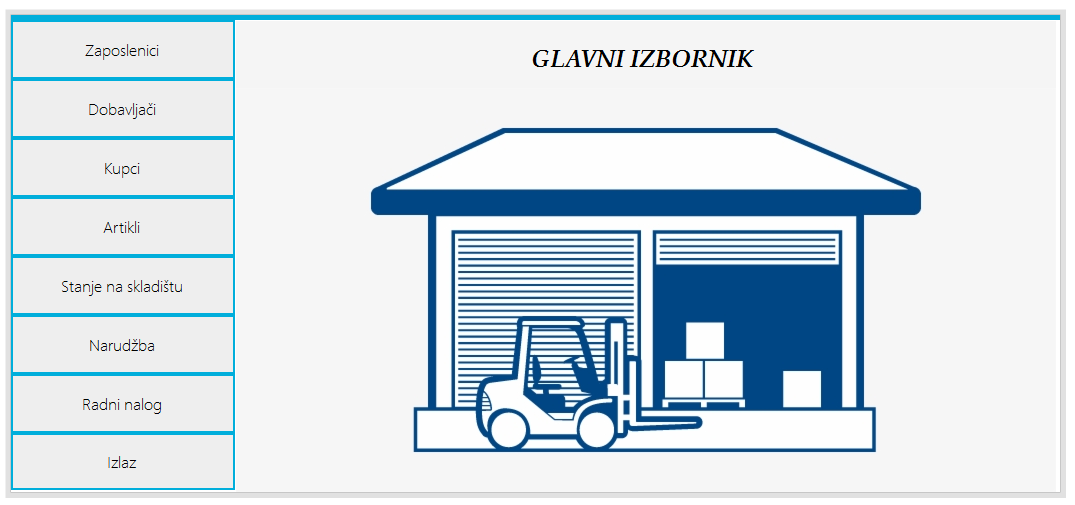
\includegraphics[width=1.0\textwidth]{slike/izbornik.PNG}
    \caption{Prikaz izbornika aplikacije}
    \label{slika-9}
\end{figure}

\section{Artikl}
Prilikom unosa artikla potrebno je popuniti sva ponuđena polja, pri čemu je potrebno ukupnu količinu postaviti na 0. Kasnije će se unosom narudžbe ili radnog naloga ukupna količina povećavati, odnosno smanjivati. Na slici 10. vidljiv je prikaz svih unesenih artikala.
\begin{figure}[h]
    \centering 
    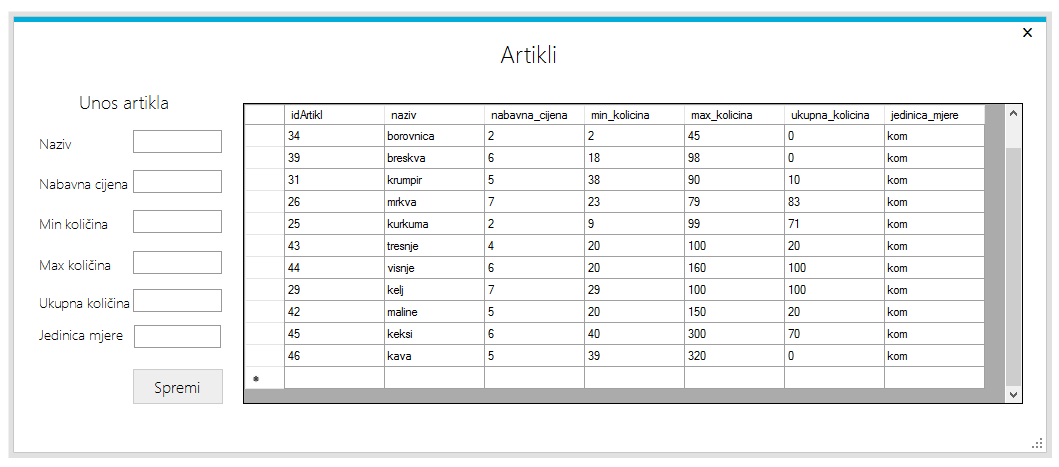
\includegraphics[width=1.0\textwidth]{slike/prikaz unesenog artikla.PNG}
    \caption{Prikaz unesenih artikala}
    \label{slika-10}
\end{figure}
\newpage
\section{Narudžba}
U prvoj tablici na formi Narudžba vidljivi su svi artikli koje je moguće naručiti dok je na drugoj tablici prikazan popis svih narudžba. Selektiranjem npr. artikla kave i pritiskom na gumb "Unos narudžbe" otvara se nova forma "Unos narudžbe". Na toj formi moguće je odabrati koji zaposlenik izdaje narudžbu, od kojeg dobavljača, na koji datum i količinu koju želi naručiti, kao i opis narudžbe koji nije obavezan za unijeti. Važno je za napomenuti da se ne može unijeti količina koja je manja od definirane minimalne količine i maksimalne količine tog artikla. Isto je implementirano s 2 okidača koji je prikazan u poglavljima 4.3.1. i 4.3.2.
\begin{figure}[h]
    \centering 
    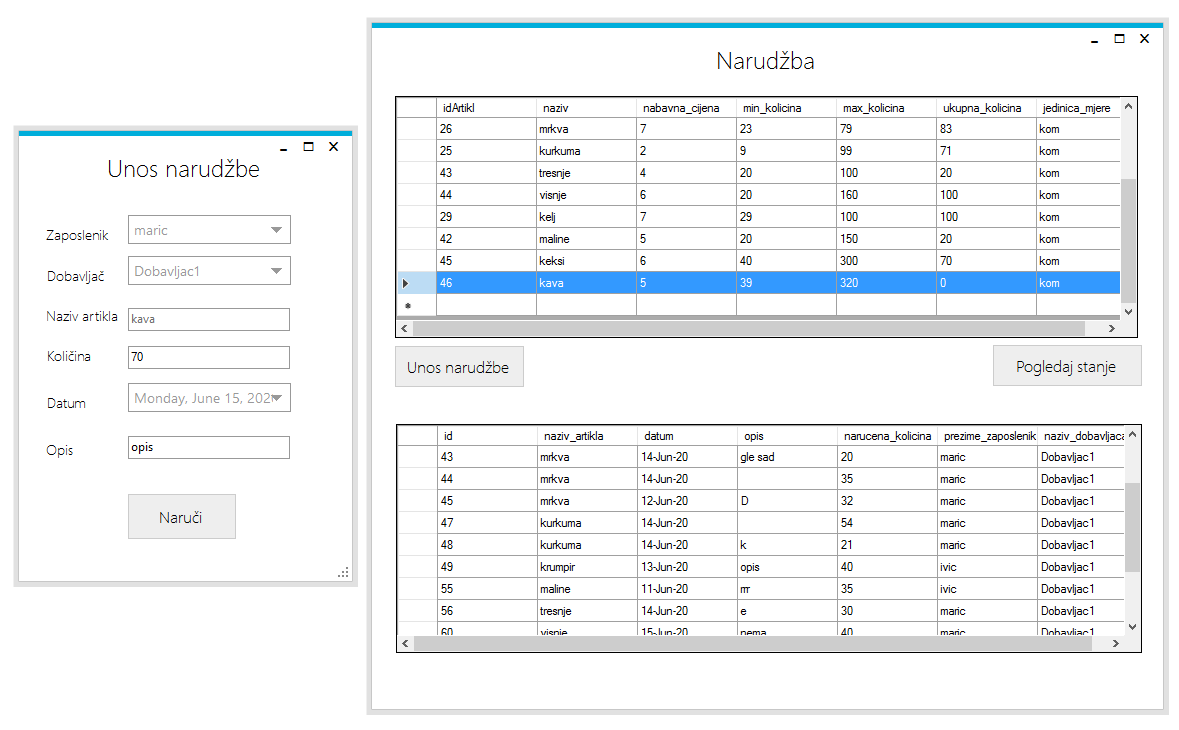
\includegraphics[width=1.0\textwidth]{slike/unos narudzbe kave.PNG}
    \caption{Prikaz unosa narudžbe}
    \label{slika-11}
\end{figure}

\section{Radni nalog}
Na slici 12. prikazan je početni izgled forme Radni nalog. Odabirom artikla u padajućem izborniku prikazuju se svi paketi tog artikla, u ovom slučaju svi paketi kave. Osim prijašnje unesenog paketa od 70 komada, izvršila se narudžba za još jedan paket od 40 komada. Obzirom da je korištena FIFO strategija, svi paketi kave su sortirani po datumu tako da je prvi prikazani paket onaj koji je prvi naručen, odnosno koji je najstariji. Na slici 12. vidljivo je kako je za prvi paket moguće izdati radni nalog, odnosno omogućen je pritisak na gumb "Izdaj nalog". Nakon unesene količine od 40 komada javlja se poruka da je nalog uspješno izdan.
\newpage
\begin{figure}[h]
    \centering 
    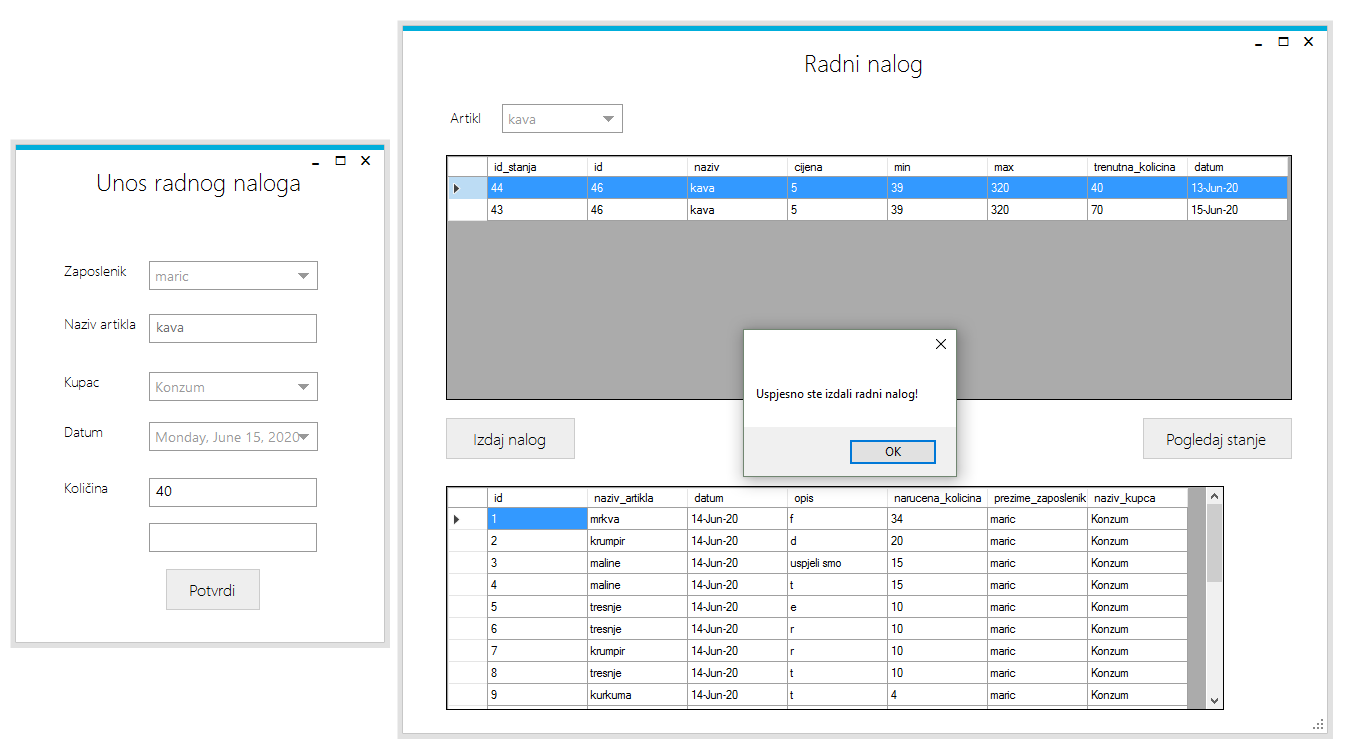
\includegraphics[width=1.0\textwidth]{slike/unos radni nalog kave.PNG}
    \caption{Prikaz unosa narudžbe}
    \label{slika-12}
\end{figure}

Međutim, ukoliko korisnik želi izdati radni nalog za drugi paket, a prvi još nije izdan, tada mu se onemogućuje pritisak na gumb "Izdaj nalog" što je vidljivo na slici 13. Na taj način zaposlenik aplikacije je primoran izdati radni nalog za prvi paket kave. Time se poštuje korištenje FIFO strategije. 

\begin{figure}[h]
    \centering 
    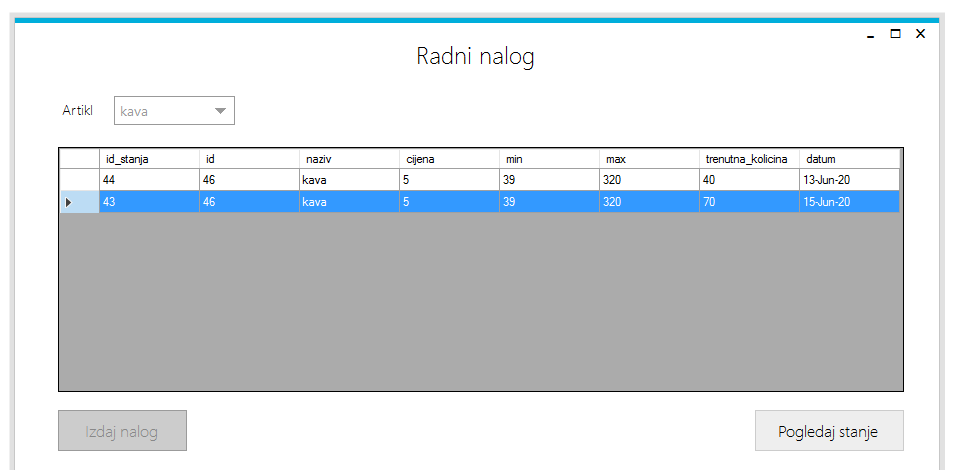
\includegraphics[width=1.0\textwidth]{slike/drugi paket kave ne moze se naruciti.PNG}
    \caption{Prikaz unosa narudžbe}
    \label{slika-13}
\end{figure}

\newpage
\section{Stanje na skladištu}
U sljedećim potpoglavljima bit će prikazano i opisano što se događa nakon što se unesu narudžba i radni nalog nekog artikla.
\subsection{Stanje nakon izdane narudžbe}
Nakon što se artikl naručio, on dospijeva na skladište gdje je vidljiva trenutna količina koja predstavlja količinu koja se naručila. Obzirom da je u poglavlju 5.2 prikazano da je naručeno 70 kavi, isto je evidentirano i na stanju na skladištu na slici 12.
\begin{figure}[h]
    \centering 
    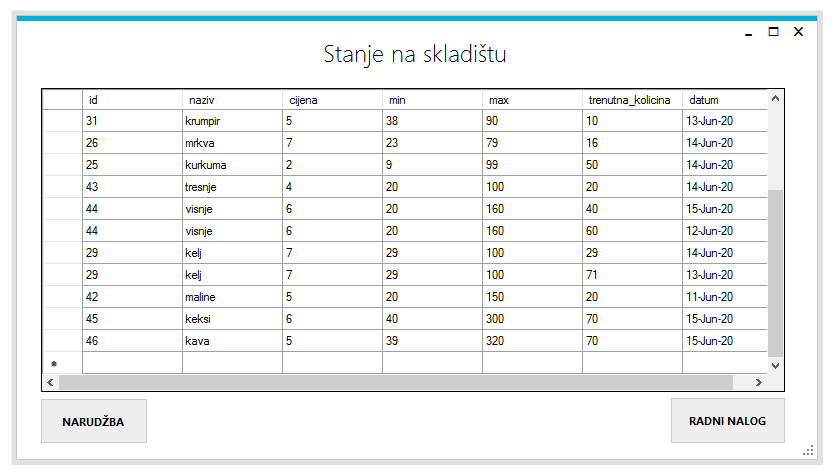
\includegraphics[width=1.0\textwidth]{slike/stanje kave.PNG}
    \caption{Prikaz stanja na skladištu nakon unesene narudžbe}
    \label{slika-14}
\end{figure}

Osim toga povećava se ukupna količina tog artikla kave na formi Artikli. Naručena su 2 paketa artikla kave, jedan od 70 komada i jedan od 40 komada pa je ukupna količina artikla kave 110. Isto je prikazano na slici 15.
\newpage
\begin{figure}[h]
    \centering 
    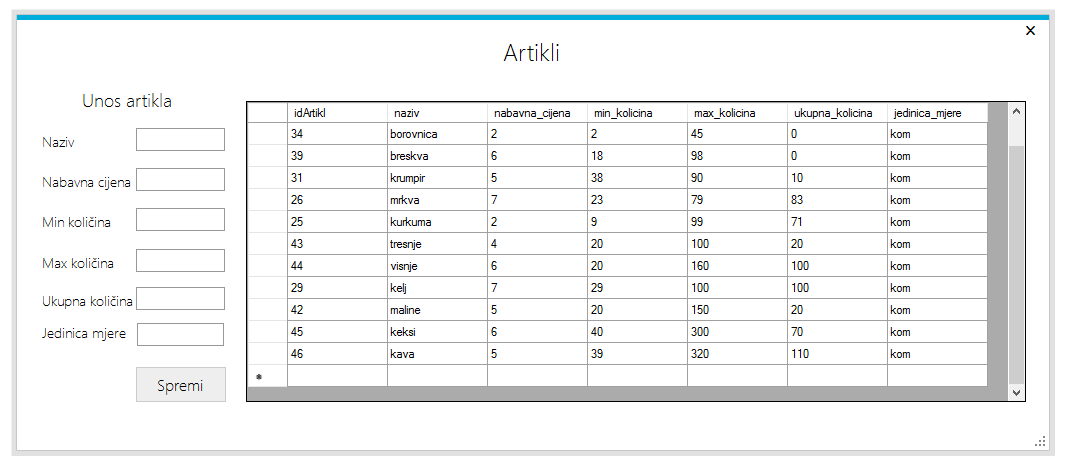
\includegraphics[width=1.0\textwidth]{slike/ukupna kol kave.PNG}
    \caption{Prikaz ukupne količine artikla}
    \label{slika-15}
\end{figure}

\subsection{Stanje nakon izdanog radnog naloga}
Nakon što se izdao radni nalog, tada mu se trenutna količina sa stanja na skladištu umanjuje za unesenu količinu u radnom nalogu. Na slici 16. vidljiva su 2 paketa, od kojih je jedan od 70 komada, a drugi ima 0 zbog izdanog radnog naloga gdje mu se smanjila količina za 40. 

\begin{figure}[h]
    \centering 
    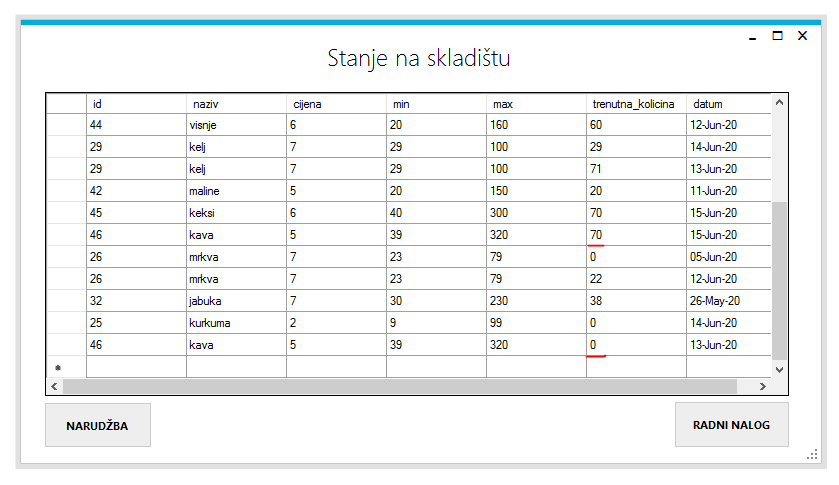
\includegraphics[width=1.0\textwidth]{slike/stanje kave nakon radnog naloga.PNG}
    \caption{Prikaz stanja na skladištu nakon izdanog radnog naloga}
    \label{slika-16}
\end{figure}
\newpage
Osim smanjivanja sa stanja na skladištu, artiklu se smanjuje i ukupna količina na formi Artikl. Vidljivo je kako se s prijašnjih 110 komada, koji su prikazani na slici 15., ukupna količina smanjila za 40, odnosno za količinu koja se prodala određenom kupcu. Isto je prikazano na slici 17.

\begin{figure}[h]
    \centering 
    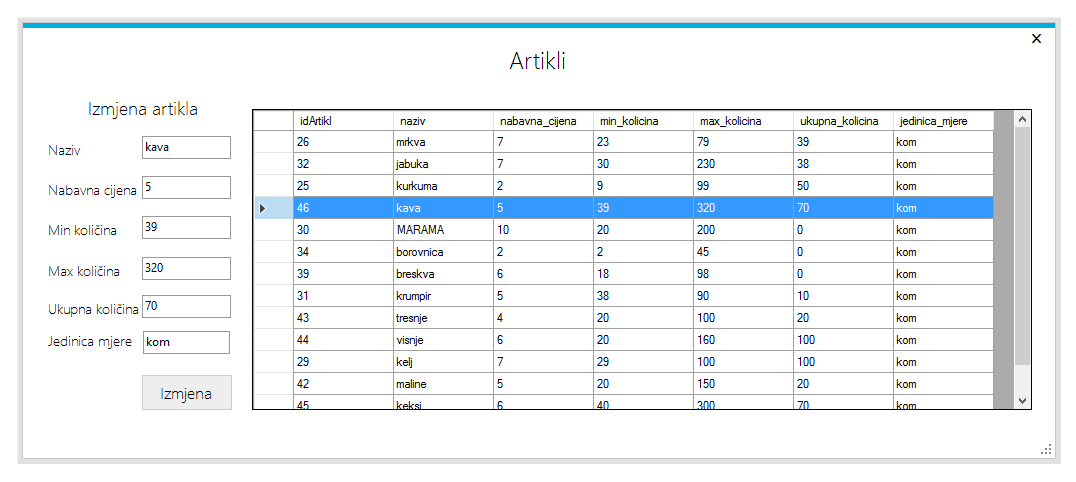
\includegraphics[width=1.0\textwidth]{slike/ukupna kol kave nakon radnog naloga.PNG}
    \caption{Prikaz ukupne količine artikla nakon izdanog radnog naloga}
    \label{slika-17}
\end{figure}
\chapter{Literatura}
[1] X.Li ,S.Chapa, J.Medina, Structural Model of ECA Rules in Active Database, 2002. godina,
Dostupno: \url{https://www.researchgate.net/publication/220887627_A_Structural_Model_of_ECA_Rules_in_Active_Database}, Preuzeto: 15.6.2020.

[2] J.Patel, Temporal Database System, 2003.godina, Dostupno:
\url{https://pdfs.semanticscholar.org/6aca/8dc7994af13f05022ce1531d99eedb64f797.pdf}, Preuzeto: 15.6.2020.

[3] FreshBooks, What is FIFO Method: Definition and Example, Dostupno: \url{https://www.freshbooks.com/hub/accounting/what-is-fifo} , Preuzeto: 15.6.2020.
\chapter{Zaključak}

Ovaj projekt izrađen je u alatu pgAdmin 4 s kojim sam se prvi put susreo. Sam alat vrlo je jednostavan za korištenje te sam se brzo snašao u njemu. Kroz samu izradu projekta prisjetio sam se PostgreSQL-a i svoje dosadašnje znanje doveo na višu razinu. Korištenje aktivnih i temporalnih baza podataka u ovoj temi ima velikog smisla jer se pomoću njih može ostvariti upravljanje zalihama. Sukladno tome okidači igraju veliku ulogu u samoj aplikaciji jer se temeljem njih događaju izračuni te se onemogućuje korisniku unos ukoliko nije zadovoljen neki uvjet. 

S druge strane, zbog odabrane FIFO strategije, bili su važni datumi ulaska proizvoda na skladište kako bi se prema njima odredilo koji artikli moraju prvo izaći van sa skladišta. Artikli istog naziva mogu imati više paketa. Samim time nije određeno da artikli različitih naziva su sortirani po datumu, već su paketi koji imaju isti naziv artikla sortirani po datumu, tako da prvi artikl koji može izaći sa skladišta je onaj najstariji.
Izrada same aplikacije nije mi predstavljala preveliki izazov jer sam se već susreo sa CSharpom i Visual Studiom u kojem je aplikacija izrađena. Na samom projektu naučio sam mnogo toga o okidačima što mi je do sada predstavljalo izazov.


\printbibliography[title=Popis literature]
\addcontentsline{toc}{chapter}{Popis literature}

\listoffigures
\addcontentsline{toc}{chapter}{Popis slika}
 

\appendix
\renewcommand{\thechapter}{\arabic{chapter}}

\end{document}
